\section{Additional Figures}
\label{sec:appendix1:add_figures}

\begin{figure}[t!]
  \begin{center}
    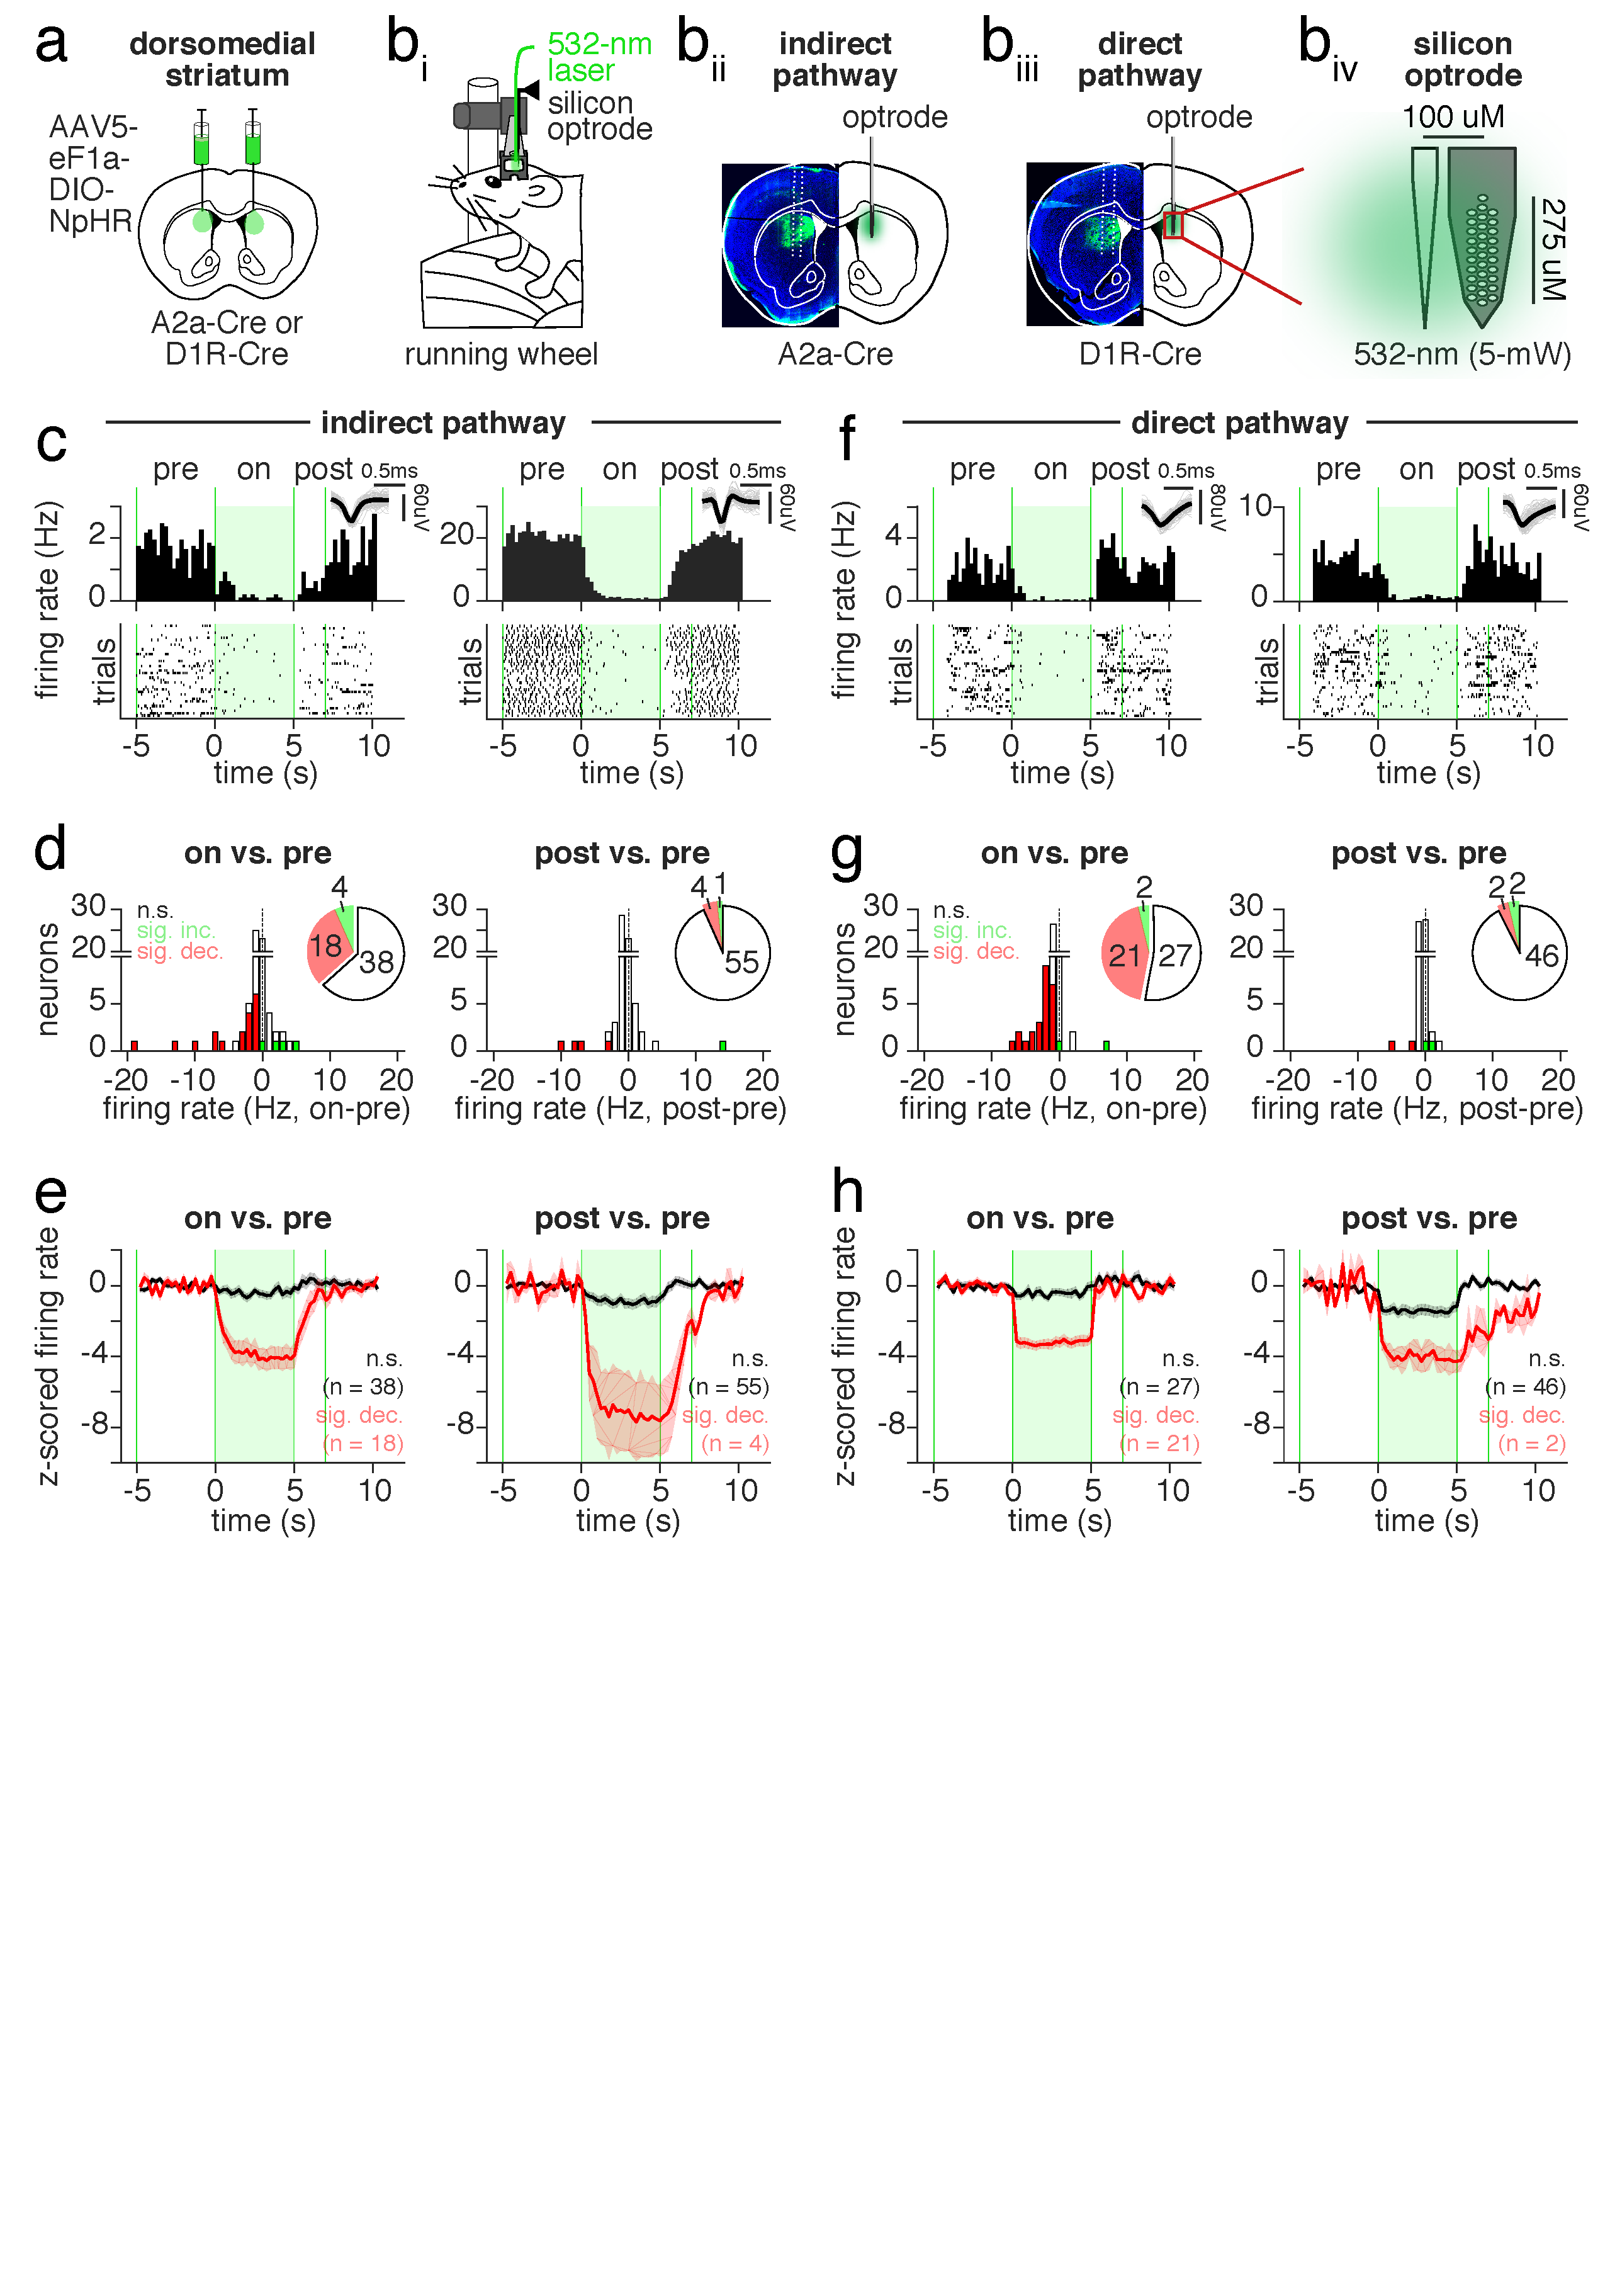
\includegraphics[width=0.90\linewidth]{ch7-appendix1/appendix1-figures/ExtData_Fig1.pdf}
    \caption[Optogenetic inhibition of DMS pathways is effective, generating little post-inhibitory rebound, nor excitation during the inhibition period]{\textbf{Optogenetic inhibition of DMS pathways is effective, generating little post-inhibitory rebound, nor excitation during the inhibition period.} (a) Schematic of viral delivery of AAV5-eF1a-DIO-NpHR to the dorsomedial striatum (DMS) of A2a-Cre or D1R-Cre mice. (b,i) Schematic of electrophysiological recording and laser delivery (532-nm, 5-mW) to the DMS in awake, head-fixed mice ambulating on a running wheel. (b,ii) Example recording electrode tracks and cre-dependent NpHR expression in an A2a-Cre mouse targeting the indirect pathway of the DMS. (b,iii) As in b,ii but in a D1R-Cre mouse targeting the DMS direct pathway. (b,iv) Schematic of silicon optrode recording tip, including tapered optical fiber coupled to a 32-channel silicon probe. (c) Two example peristimulus time histograms (PSTH) (top) and raster plots of trial-by-trial spike times (bottom) from single neurons recorded from the DMS of an A2a-Cre mouse. Inset at top displays average spike waveform (black) and 100 randomly sampled spike waveforms (grey) for each neuron. A trial consisted of 5-s without laser (pre, -5 to 0-s), 5-s of 532-nm light (5-mW) delivery (on, 0 to 5-s), followed by a 10-s ITI (40 trials per recording site). The first 2-s following laser offset (post, 5-7-s) was used to assess post-inhibitory effects. (d) Left: Histogram of change in average firing rate (on-pre, Hz) for all neurons (n = 60) recorded from the DMS of A2a-Cre mice (n = 3). Colors indicate non-significant (black, n = 38 neurons), significantly decreased }
    \label{fig:ap1:ext1}
  \end{center}
  \vspace{-1.5cm}
\end{figure}
\begin{figure}[t!]
\vspace{-7cm}
  \contcaption{(red, n = 18 neurons) or increased (green, n = 4 neurons) changes in firing rate determined via paired, two-tailed signrank comparison of average across-trial baseline (pre) or laser (on) firing rates. A Bonferroni-corrected significance threshold was used to account for multiple neuron comparisons (p < 0.00083, or p = 0.05/60 neuron comparisons). Right: same as left but for change in firing rate (post-pre, Hz): non-significant (n = 55 neurons), significantly decreased (n = 4) or increased (n = 1). Insets display pie-chart summaries of the proportion of non-significant (black unfilled), significantly decreased (red) or increased (green) neurons. (e) Left: Mean +/- SEM z-scored firing rate across all non-significantly modulated on vs pre (black, n = 38) or significantly decreased on vs pre (red, n = 18) neurons recorded from A2a-Cre mice. Right: same as left but for all non-significantly modulated post vs pre (black, n = 55) or significantly decreased post vs pre (red, n = 4) neurons. (f) Same as c but for example neurons recorded from the DMS of D1R-Cre mice. (g) Same as d but for all neurons (n = 50) recorded from the DMS of D1R-Cre mice (n = 2). Left (on-pre): non-significant (n = 27), significantly decreased (n = 21), or increased (n = 2). Right (post-pre): non-significant (n = 46), significantly decreased (n = 2) or increased (n = 2). A Bonferroni-corrected significance threshold was used to account for multiple neuron comparisons (p < 0.001, or p = 0.05/50 neuron comparisons). (h) same as e but for neurons recorded from the DMS of D1R-Cre mice.}% Continued caption
\end{figure}

\begin{figure}[t!]
  \begin{center}
    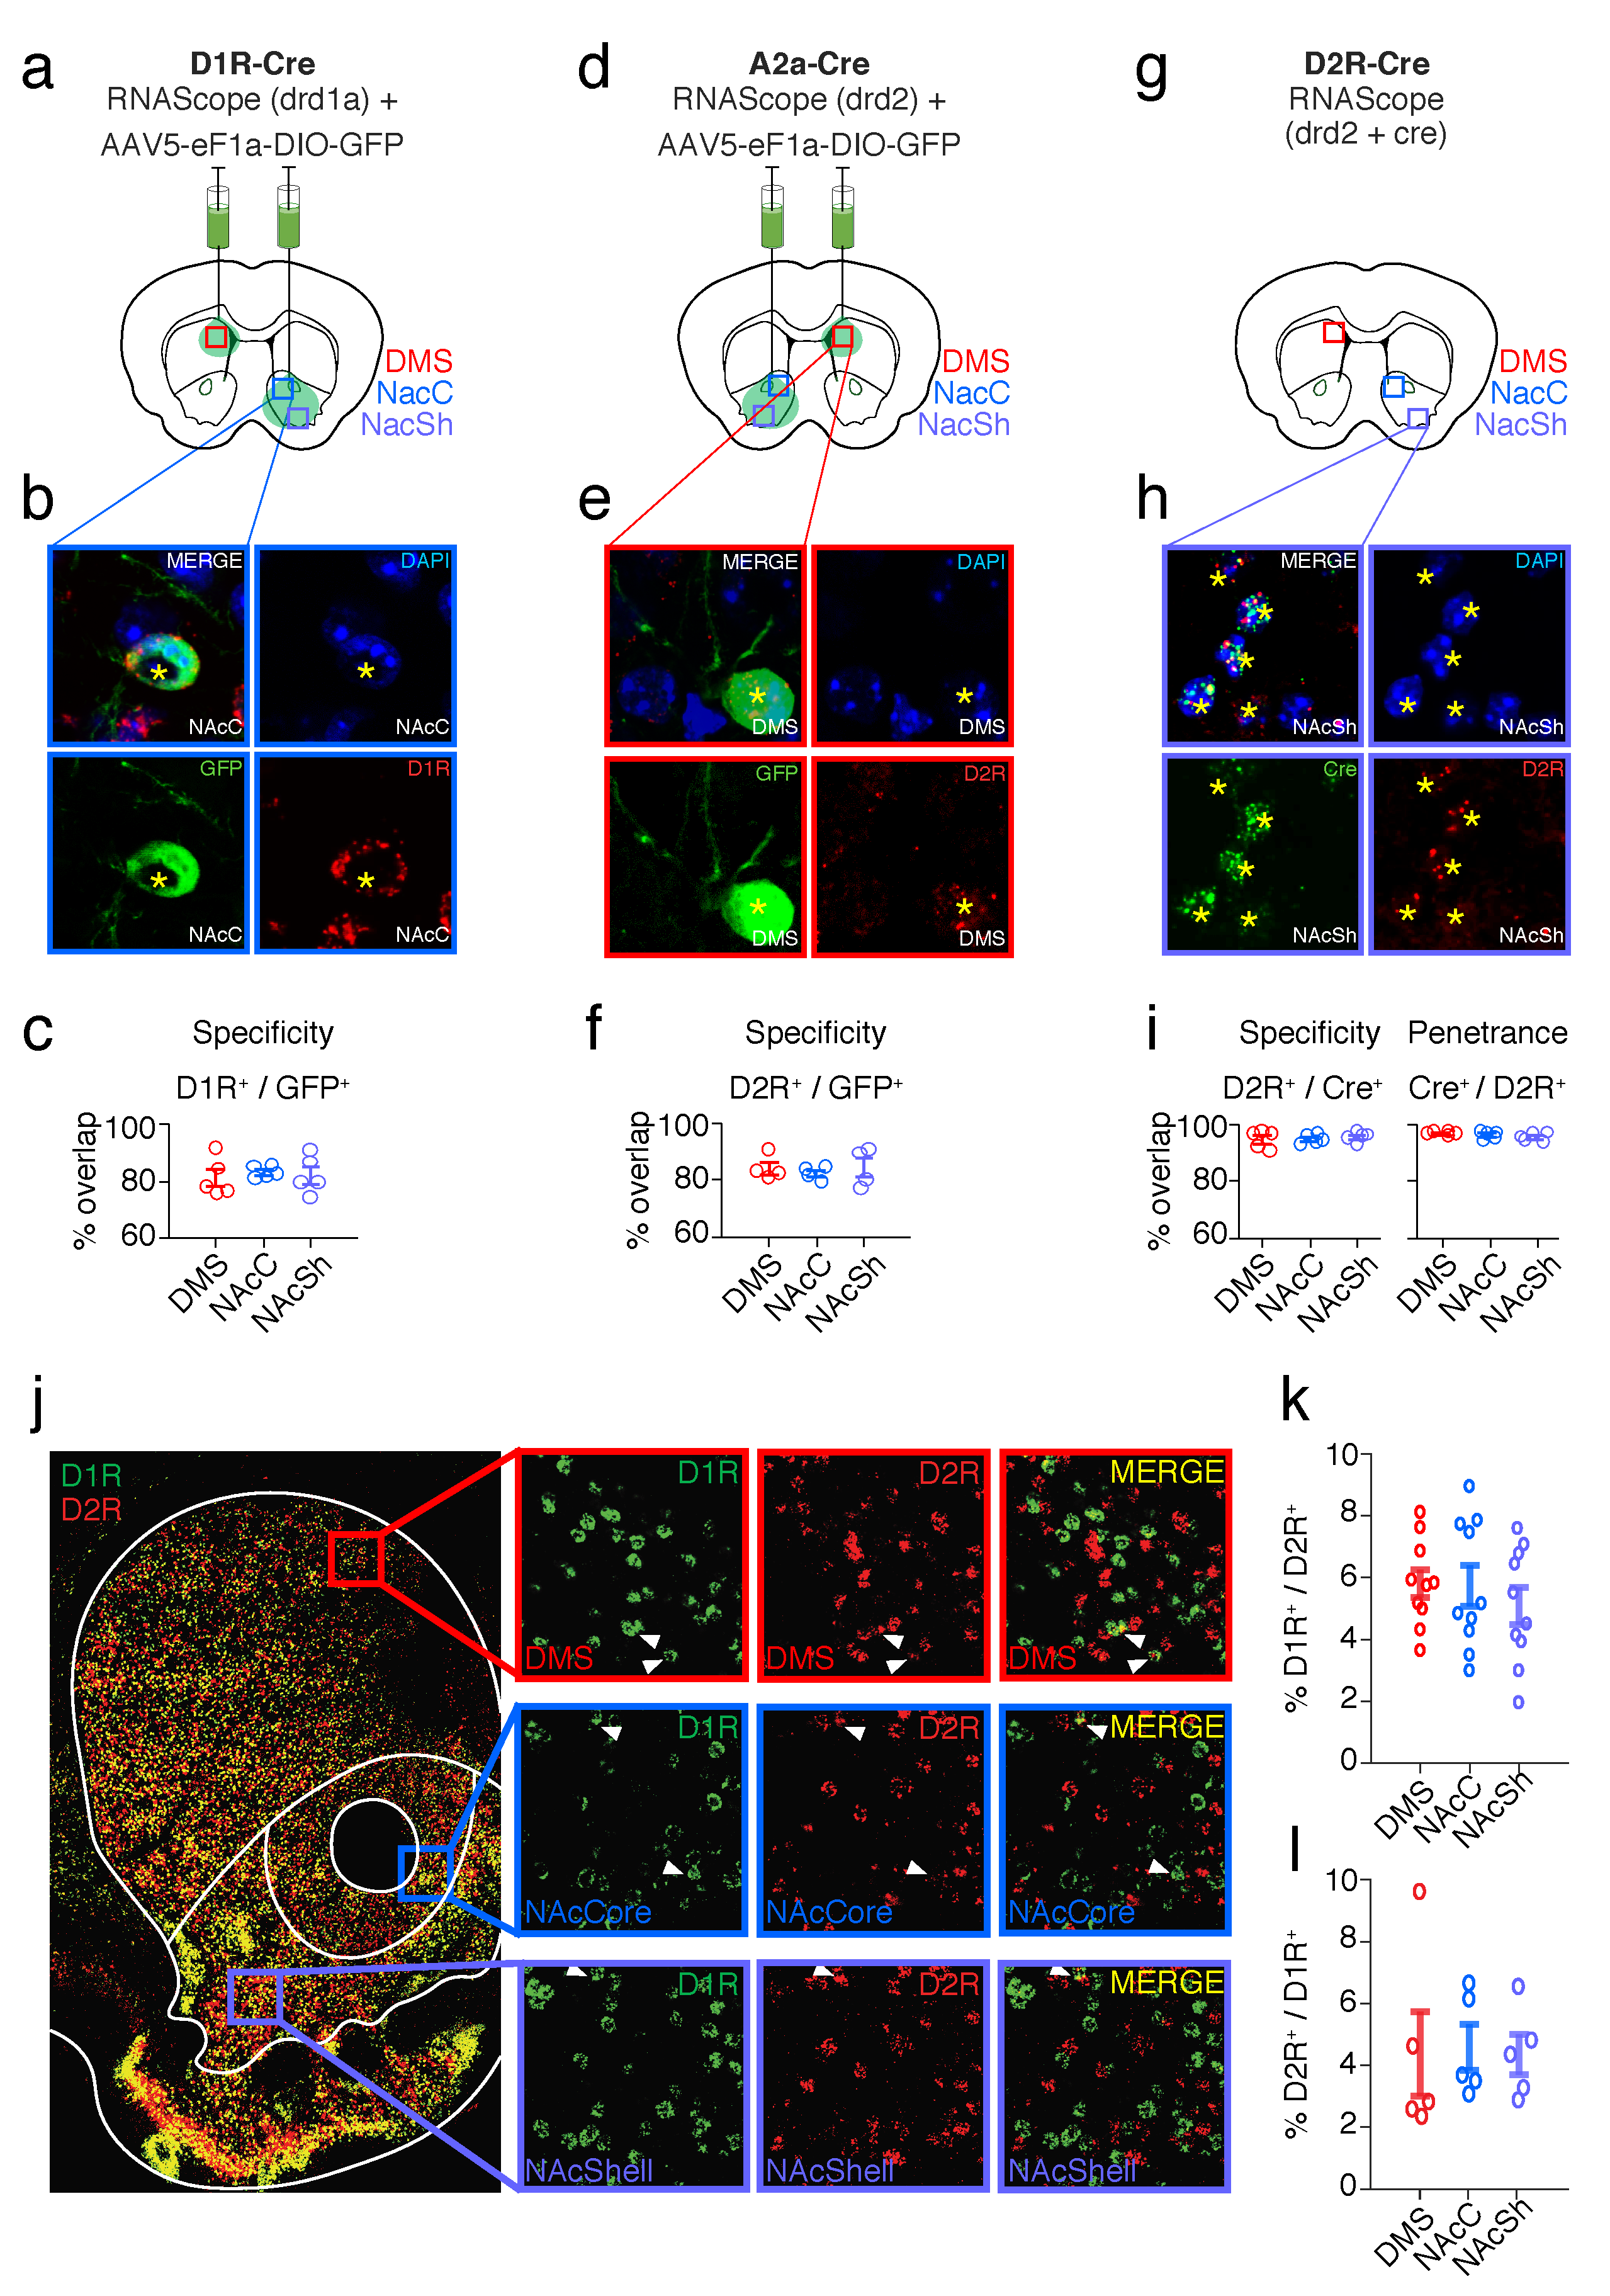
\includegraphics[width=0.90\linewidth]{ch7-appendix1/appendix1-figures/Supplementary_Fig1.pdf}
    \caption[Transgenic mouse lines faithfully report indirect and direct pathways across striatal subregions]{\textbf{Transgenic mouse lines faithfully report indirect and direct pathways across striatal subregions.}}
    \label{fig:ap1:supp2}
  \end{center}
  \vspace{-1.5cm}
\end{figure}
\begin{figure}[t!]
  \contcaption{(a) Schematic of viral delivery of AAV5-eF1a-DIO-GFP to the dorsomedial striatum (DMS) or nucleus accumbens (NAc) on opposite hemispheres of D1R-Cre mice. Red, blue, and purple squares denote representative areas for stereological quantification of viral co-expression with a drd1 mRNA probe (RNAScope) in the DMS, NAc core (NAcC), or NAc shell (NAcSh), respectively. (b) Example fluorescent confocal image (63x objective, 5x digital zoom) of the NAc core from a D1R-Cre mouse displaying virally- expressed GFP (green), drd1 mRNA (red), and DAPI (blue). (c) Percentage of GFP+ neurons co-expressing drd1 mRNA from 2 D1R-Cre mice across the DMS (red; n = 5 sections; 193 GFP+ neurons), NAcC (blue; n = 5 sections; 298 GFP+ neurons), or NacSh (purple; n = 4 sections; 312 GFP+ neurons). (d) Same as a, but for quantification of viral co-expression with a drd2 mRNA probe in A2a-Cre mice. (e) Same as b, but for an example image of the DMS from an A2a-Cre mouse and displaying drd2 mRNA (red). (f) Same as c, but for percentage of virally-expressed GFP+ neurons co-expressing drd2 mRNA in 2 A2a-Cre mice across the DMS (red; n = 4 sections; 312 GFP+ neurons), NAcC (blue; n = 4 sections; 326 GFP+ neurons), or NacSh (purple; n = 4 sections; 312 GFP+ neurons). (G) Same as A and D, but for quantification of co-expression of drd2 and cre mRNA in 2 D2R-Cre mice. (h) Same as b and e, but for an example image of the NAcSh from a D2R-Cre mouse and displaying cre mRNA (green) and drd2 mRNA (red). (i) Left: same as c and f, but for percentage of neurons with cre mRNA co-expressing drd2 mRNA in 2 D2R-Cre mice across the DMS (red; n = 5 sections; 1302 cre+ neurons), NAcC (blue; n = 5 sections; 1,104 cre+ neurons), or NacSh (purple; n = 4 sections; 1,187 cre+ neurons). Right: same as left but for neurons with drd2 mRNA co-expressing cre mRNA across DMS (red; n = 5 sections; 1,269 drd2+ neurons), NAcC (blue; n = 5 sections; 1,055 drd2+ neurons), or NacSh (purple; n = 5 sections; 1,114 cre+ neurons). Solid bars denote mean and s.e.m. throughout. (j) Example fluorescent confocal microscopy image of a coronal section from a DR2-Cre mouse that underwent fluorescent in situ hybridization with probes targeting drd1a and drd2 receptor mRNA. Left: 20x magnification tilescan spanning dorsal and ventral striatum. Right top: 63x confocal images of dorsomedial striatum (DMS, red square) and expression of drd1a mRNA (green), drd2 mRNA (red), and merged image of both (yellow). White triangles indicate co-expression of receptor probes in single neurons. Right middle: same as right top but for 63x confocal images of nucleus accumbens core (NAcC, blue square). Right bottom: same as right top but for 63x confocal images of nucleus accumbens shell (NAcSh, purple square). (k) Percentage of drd2+ neurons co-expressing drd1a mRNA from 2 D2R-Cre and 2 D1R-tdTomato mice in the DMS (red; n = 10 sections; 2,423 drd2+ neurons), NAcC (blue; n = 10 sections; 2,196 drd2+ neurons), or NacSh (purple; n = 10 sections; 2,220 drd2+ neurons). Circles indicate mean overlap from individual sections. (l) Same as k, but for percentage of drd1a+ neurons co-expressing drd2 mRNA from 2 D1R-tdTomato mice in the DMS (red; n = 5 sections; 868 drd1a+ neurons), NAcC (blue; n = 5 sections; 834 drd1a+ neurons), or NacSh (purple; n = 5 sections; 874 drd1a+ neurons). Throughout solid bars reflect mean +/- S.E.M. and transparent ‘o’ denote individual slice mean. Each staining was repeated on 2 independent samples (mice) per group with similar results.  }% Continued caption
\end{figure}

\begin{figure}[t!]
  \begin{center}
    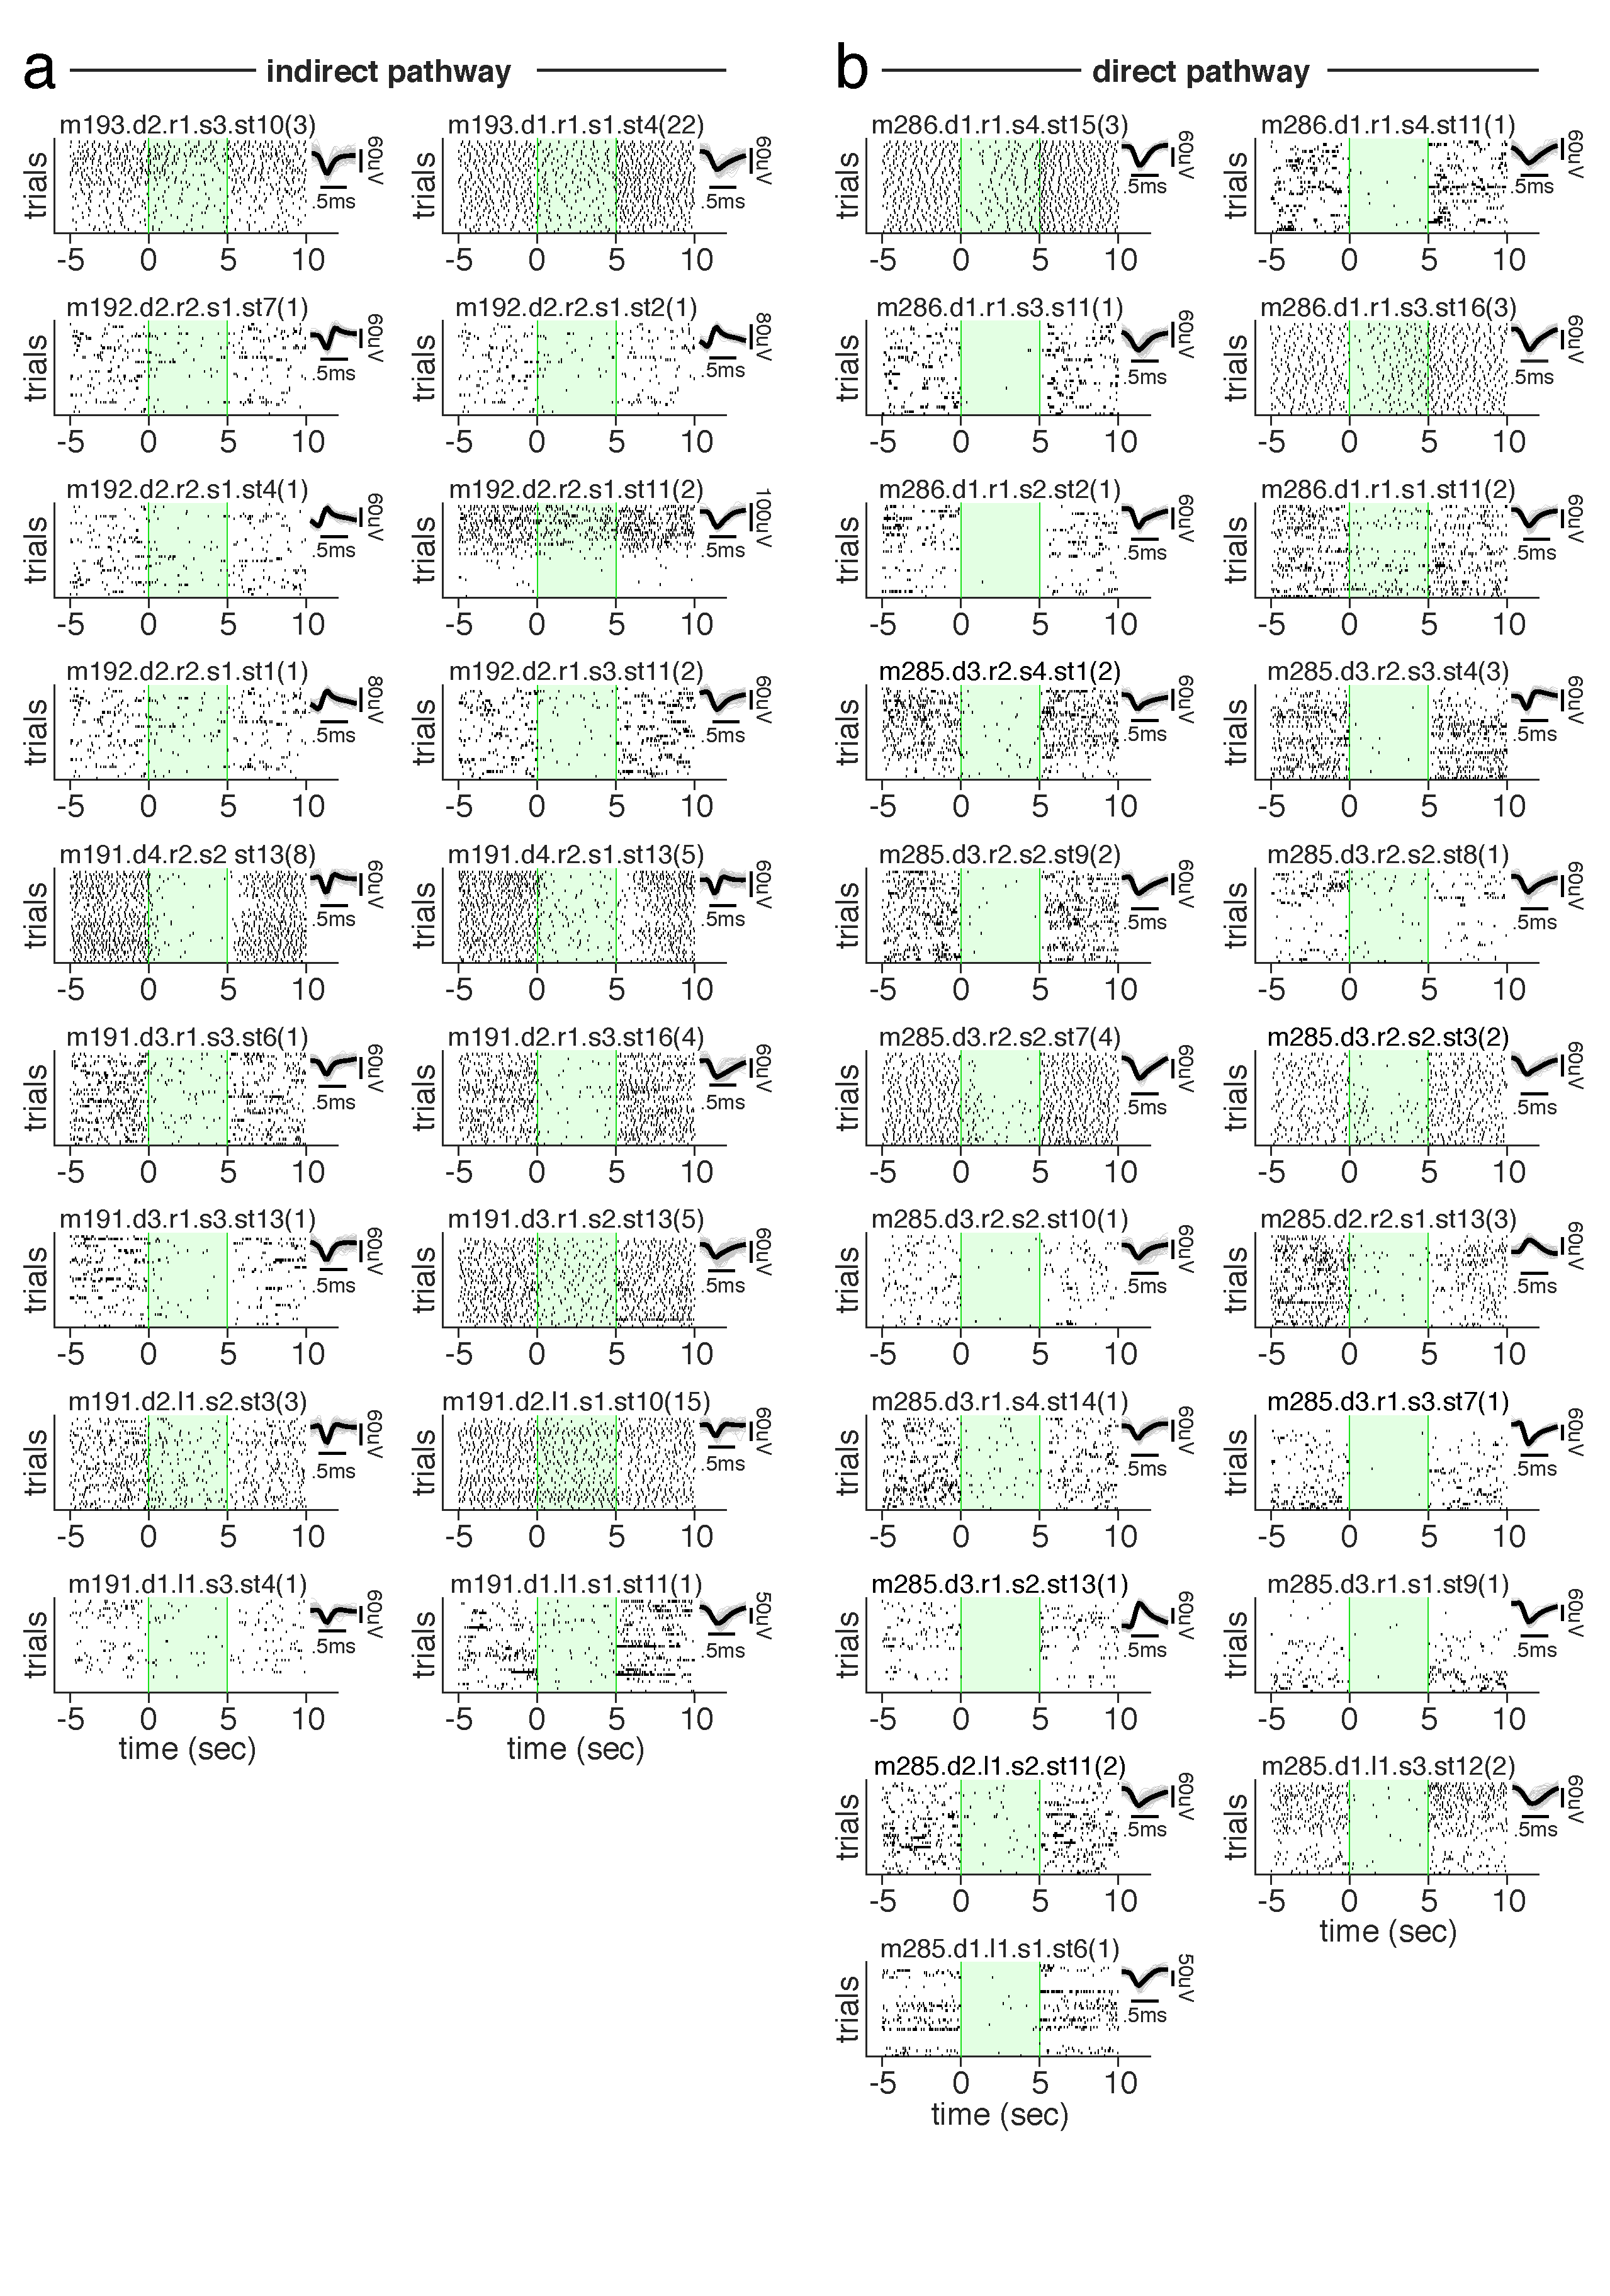
\includegraphics[width=0.90\linewidth]{ch7-appendix1/appendix1-figures/Supplementary_Fig2.pdf}
    \caption[Indirect and direct pathway inhibition of the DMS is stable across time]{\textbf{Indirect and direct pathway inhibition of the DMS is stable across time.} }
    \label{fig:ap1:ext1}
  \end{center}
  \vspace{-1.5cm}
\end{figure}
\begin{figure}[t!]
\vspace{-3cm}
  \contcaption{\textbf{}  (a) Trial-by-trial raster plots of single neuron spiking during laser off baseline (-5 to 0s), 532-nm  (5-mW)  laser delivery (0 to 5s), and post laser offset (5 to 10s) for all significantly inhibited neurons  (n = 18/60) recorded from A2a-Cre mice expressing Cre-dependent NpHR in the DMS. 40 total trials of laser sweeps per recording site (~15 minutes), ordered in time top to bottom. Individual neuron labels indicate: m (mouse), d (day of recording), r/l (right/left hemisphere and penetration number), s (site or depth of recording probe numbered ventral to dorsal), and st (probe stereotrode channel). Number in parenthesis indicates the number of spikes sub-sampled for display. Inset displays average (bold) and 100 randomly sampled spike waveforms (grey). (b) As in a but for all significantly inhibited neurons recorded from D1R-Cre mice expressing Cre-dependent NpHR in the DMS (n =21/50).}% Continued caption
\end{figure}